\documentclass[12 pt, a4paper]{report}
%\documentclass[runningheads]{llncs}
\usepackage[T1]{fontenc}
\usepackage{mathptmx}
\usepackage{amsmath,amssymb,amsfonts, amsthm}

\theoremstyle{definition}
\newtheorem{definition}{Definition}[section]

\usepackage{setspace}
%\usepackage[top=1 in,bottom=1 in,left=3.2 cm,right=2.6 cm]{geometry}
\usepackage[utf8]{inputenc}
\usepackage{fullpage}
\usepackage{graphicx}
%\renewcommand{\baselinestretch}{2}
\renewcommand{\thesection}{\arabic{section}}
%\raggedbottom
\usepackage[sort&compress,numbers]{natbib}
\usepackage[hidelinks]{hyperref}
\usepackage[nottoc]{tocbibind}
\usepackage{rotating}
\usepackage{hyperref}
\usepackage{lipsum}
\usepackage{xcolor}
%\usepackage{afterpage}
\usepackage{parskip} 
%removes indentation but gives some spacing ebtween para
\usepackage{todonotes}

\usepackage{listings}

\definecolor{codegreen}{rgb}{0,0.6,0}
\definecolor{codegray}{rgb}{0.5,0.5,0.5}
\definecolor{codepurple}{rgb}{0.58,0,0.82}
\definecolor{backcolour}{rgb}{0.95,0.95,0.92}

\lstdefinestyle{mystyle}{
    backgroundcolor=\color{backcolour},   
    commentstyle=\color{codegreen},
    keywordstyle=\color{magenta},
    numberstyle=\tiny\color{codegray},
    stringstyle=\color{codepurple},
    basicstyle=\ttfamily\scriptsize,
    breakatwhitespace=false,         
    breaklines=true,                 
    captionpos=b,                    
    keepspaces=true,                 
    numbers=none,                    
    numbersep=5pt,                  
    showspaces=false,                
    showstringspaces=false,
    showtabs=false,                  
    tabsize=2,
    escapechar=\%
}

\lstset{style=mystyle}



\newcommand{\blankpage}{
\newpage
\thispagestyle{empty}
\addtocounter{page}{-1}
\mbox{}
\newpage
}

%\newcommand\blankpage{%
%    \null
%    \thispagestyle{empty}%
%    \addtocounter{page}{-1}%
%    \newpage}

%\def\keywords{\vspace{.5em}
%{\textit{Keywords}:\,\relax%
%}}
%\def\endkeywords{\par}

%\providecommand{\keywords}[1]
%{
%  \small	
%  \textbf{\textit{Keywords---}} #1
%

\newcommand{\lukas}[1]{\todo[inline,color=green]{#1}}




\onehalfspacing
\begin{document}
%\maketitle
\sloppy
\begin{titlepage}

	\begin{doublespace}

% 		\begin{flushleft} 
 
			
\includegraphics[width=0.4\textwidth]{images/logo.jpg}

			\hrule
			\vspace*{0.15cm}
			{\Large Faculty of Computer Science}
			\vspace*{0.15cm}
			\hrule

%    \begin{center}
		\begin{center}
        		\vspace{1cm}      
        
       		{\LARGE \textbf{Master Thesis} }
            
        		\vspace{0.25cm}
        
        		{\Large \textbf{Querying Wikidata with GraphQL} 
%			(Wikidata mit GraphQL Abfragen) 
			}
            
        		\vspace{1.5cm}
        \end{center}
        
        
%	 \begin{flushleft}
			Anas Shahab \\
    			Master Computational Logic \\
    			Matriculation number: 4827407
    		
    			\vspace{0.5cm}
    		
    			Supervisor: \\
	    		Prof. Dr. Markus Kr{\"otzsch}
    			
    			\vspace{0.25cm}
    		
    			Second Reviewer: \\
			Dr. Dörthe Arndt
    			
    			\vspace{0.25cm}
    		
    			
    			Tutor: \\
    			Dipl.-Inf. Lukas Gerlach
    		
    			\vspace{0.5cm}
    		
    			Faculty of Computer Science \\
    			Institute of Theoretical Computer Science \\
    			Chair of Knowledge-Based Systems
    		
    			\vspace{1cm}
    		
    			Submission Date: \textcolor{red}{XX.XX.2023}
    			
%		\end{flushleft}
                  
	\end{doublespace}
	
%	\afterpage{\blankpage}
            
%    \end{center}
\end{titlepage}
\blankpage
%\afterpage{\blankpage}

%\thispagestyle{empty}
\pagenumbering{roman}
\section*{Declaration of originality}
I hereby declare that I have written this Thesis on my own accord and any participation of others has been acknowledged. I have clearly marked all references to existing work. I have not submitted this work partly or as a whole anywhere else. \\

Dresden, XX.XX.XXXX \\
\rule{150 px}{0.5 px} \\
(signature)
\blankpage
%\afterpage{\blankpage}

%\thispagestyle{empty}
\section*{Acknowledgements}
\lipsum[1]
\blankpage

%\begin{abstract}
%\lipsum[1]
%\\[0.5 cm]
%\centerline{\keywords{x, y, z}}
%
%\end{abstract}

\section*{Abstract}
\lipsum[1]

%\pagenumbering{roman}
\tableofcontents
%\listoffigures
%\listoftables
\pagebreak

%\doublespacing
\pagenumbering{arabic}
\section{Introduction}

The term "knowledge graph" gained popularity in 2012 when Google launched its own \textit{Google Knowledge Graph}. A knowledge graph is a collection of data represented as a graph. The collected data conveys knowledge of the real world, where the nodes represent entities of interest and edges the many different relations between those entities \cite{Hogan2021}. The entities are real world objects and abstract concepts. For example, "Helium has the chemical formula He", is a statement that can be represented using a knowledge graph. Here the nodes of the graph would represent "Helium" and "He", while the connecting edge between those nodes would represent the relation "chemical formula". 

There are many ways of modelling data as a graph. The most commonly used ones are directed edge-labelled graphs, heterogeneous graphs, property graphs and graph dataset \cite{Hogan2021}. We will see in Section 2 how we can use RDF to specify directed edge-labelled graphs.

The term knowledge base is used synonymously with knowledge graph but there is a small difference \cite{Ji2022}. Normally, a knowledge graph is viewed as a graphical structure. However, when defined semantically, it is considered to be a knowledge base for interpretation and inference from facts \cite{Bordes2011}. 

Many companies such as Amazon, Facebook, Uber, Google, etc., use knowledge graphs for their applications. Depending on the organization or community there are open or enterprise knowledge graphs \cite{Hogan2021}. Open knowledge graphs include Wikidata, DBpedia, Freebase, YAGO, etc. These are available online and freely accessible to the public. Enterprise knowledge graphs are generally used internally within a company and have their commercial specific use-cases \cite{Hogan2021}.

The remainder of the report is structured as follows. In section 2, we provide an overview of RDF, Wikidata, \todo{Query language (only SPARQL) mentioned in the structure here} SPARQL and GraphQL which will be crucial in the later sections. We also give a comparison between SPARQL and GraphQL. Section 3 gives the approaches used to query RDF graphs. The implementation of the approaches on Wikidata, along with the technicalities, and the differences in the SPARQL queries generated by the tools is provided in Section 4. The differences between the generated SPARQL queries and handwritten SPARQL queries is also shown here. This section also includes the performance and limitations of the tools. Lastly, we provide a conclusion and future work in Section 5.

\section{Preliminaries}
\subsection{RDF}
The Resource Description Framework (RDF) is a framework used to represent information available in the Web \cite{R.Cyganiak2014}. In the context of graphs, RDF is used for describing and exchanging graphs. The graphs specified by RDF are directed edge-labelled graphs. This means that the edges connect source nodes to target nodes, and have labels. It can be the case that there are multiple edges between the same nodes. However, these edges must have different labels. Figure~\ref{fig:figure 1} shows how knowledge about the chemical element Helium can be represented using directed edge-labelled graphs.

\begin{figure}[t]
  \centering
  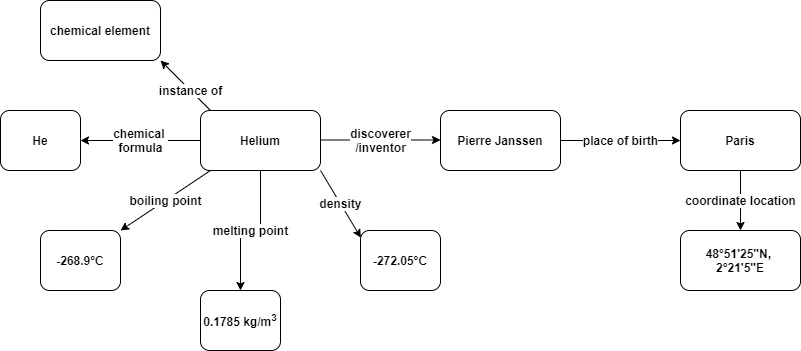
\includegraphics[width=0.75 \linewidth]{images/del_graph.jpg}
  \caption{Directed edge-labelled graph describing Helium}
  \label{fig:figure 1}
\end{figure}

The graph shown in Fig 1 can be represented in an RDF graph. Formally, the building blocks of RDF graphs are IRIs, literals and blank nodes. They are defined as follows.

\subsubsection{IRIs}
To identify resources on the Web uniquely we use Uniform Resource Identifiers (URIs). An URI is a sequence of a subset of ASCII characters that have a scheme, authority, path, and optional query and fragment. An Internationalized Resource Identifier (IRI) is a generalized form of URI that helps to distinguish resources with Unicode. In RDF, an IRI is used as a name, or an equivalent of ID, for graph nodes \cite{Tehnologies2022}. Andy Seaborne has a good article that explains URIs and IRIs in detail \cite{Seaborne2020}.

\subsubsection{RDF Literals}

An RDF literal consists of three essential elements: a lexical value, a datatype IRI and an optional language tag. The lexical value is a string (footnote: RDF is based on Unicode strings) that corresponds to a particular literal value in the value space, where value space is the set of all possible values that a datatype can have. There are many datatypes in RDF some of which are string, Boolean, decimal and integer. A full list is available on the W3C's section on RDF datatypes: www.w3.org/TR/2014/REC-rdf11-concepts-20140225/\#section-Datatypes \textcolor{red}{should I give as footnote?}.
\lukas{yes, put the sentence with the link as footnote :)}

The datatype IRI refers to a datatype that defines which strings are valid (belong in the lexical space), the value space and the lexical-to-value mapping \cite{ Bonduel2019}. This mapping is essentially a function that maps each string from the lexical space to an element in the value space. The W3C  standard XML Schema defines the datatypes and their IRIs. For example, decimals are identified by the IRI http://www.w3.org/2001/XMLSchema\#decimal. W3C has a good documentation on the different XML Schema built-in datatypes \cite{ R.Cyganiak2014}.

The optional language tag helps to provide human-readable labels to RDF literals. A literal is a language-tagged string is of the form "string"@language (footnote: language is a well-formed language tag (after BCP47). The datatype IRI of such literals is http://www.w3.org/1999/02/22-rdf-syntax-ns\#langString (footnote: It is never used in syntax).


RDF literals are used to represent resources that have values belonging to datatypes. Each literal can have only one datatype. For example, the boiling point of Helium would be a RDF literal represented as \todo{change font}-268.9^^xsd:decimal and its chemical formula as \todo{change font}"He"@en, which is a language-tagged string. 

\subsubsection{Blank Nodes}
Unlike an IRI or a literal, a blank node does not identify some specific resource \cite{ R.Cyganiak2014}. It is used as a placeholder for some node, i.e., it is used to say that something with the given relationship exits at the position without specifying what the node is.

\begin{definition}[RDF Graph]
An RDF graph is a set of triples that consists of the following elements: 

\begin{itemize}
	\item a subject (node) that is an IRI or a blank node; 
	\item a predicate (edge) that is an IRI; 
	\item an object (node) that is an IRI, a blank node, or a literal. 
\end{itemize}	
\end{definition}

Figure~\ref{fig:figure 2} shows what an RDF graph could look like taking our example represented in Figure~\ref{fig:figure 1}. We have added a label predicate to identify Helium. Our main interest is in querying the knowledge graph Wikidata, and so all the data correspond to the resources in its knowledge base. Literals are drawn as rectangular nodes. Here wd is a prefix for http://www.wikidata.org/entity/ and wdt for http://www.wikidata.org/prop/direct/. In Wikidata items (nodes) and properties (predicates) are identified uniquely by an entity ID. Table~\ref{tab: table 1} helps to understand the RDF graph in Figure~\ref{fig:figure 2} better.

\begin{figure}[t]
  \centering
  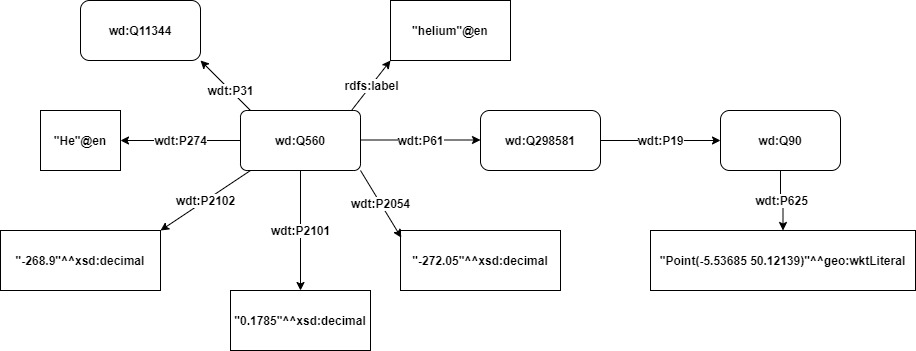
\includegraphics[width=0.75 \linewidth]{images/rdf_graph.jpg}
  \caption{RDF graph describing Helium}
  \label{fig:figure 2}
\end{figure}

\begin{table}[b!]
	\begin{center}
		\caption{Abbreviation/IDs and their meanings.}
		\label{tab: table 1}
		\begin{tabular}{c|c}
%			\textbf{Benchmarking tool} & \textbf{Resource monitoring tool} & \textbf{License} & \textbf{Updated} \\ \hline
			wd & http://www.wikidata.org/entity/ \\ \hline
			wdt & http://www.wikidata.org/prop/direct/ \\ \hline
			rdfs & http://www.w3.org/2000/01/rdf-schema\# \\ \hline
			Q560 & Helium \\ \hline
			Q298581	& discoverer/inventor \\ \hline
			Q90 & Paris \\ \hline
			P31	& instance of \\ \hline
			P274 & chemical formula \\ \hline
			P2102 & boiling point \\ \hline
			P2101 & melting point \\ \hline
			P2054 & density \\ \hline
			P61	& discoverer/inventor \\ \hline
			P19	 & place of birth \\ \hline
			P625 & coordinate location
		\end{tabular}
	\end{center}
\end{table}
\lukas{maybe table 1 could go into an appendix}

From Table~\ref{tab: table 1} we can see that wd:Q560 is an abbreviation for the IRI http://www.wikidata.org/entity/Q560, where Q560 is the entity ID for Helium. The IRI helps is to identify the resource Helium on Wikidata. The rest of the nodes and edges in Figure~\ref{fig:figure 2} can be understood analogously. We can also see that for labelling we use rdfs:label which is used to give a human-readable version of a resource's name \cite{Brickley2014} . Also, geo:wktLiteral (http://www.opengis.net/ont/geosparql\#wjktLiteral) is a datatype for representing geographic coordinates.

So far, we have shown an abstract syntax of RDF. For exchanging graphs, we need to have a concrete syntactic representation to encode RDF graphs \cite{Kroetzsch2020}.
\lukas{``RDF Graphs are often syntactically respresented in formats like...'' (leave away the introductory sentence; be more succinct)}
The most relevant formats are N-Triples, Turtle, JSON-LD, RDF/XML and RDFa. W3C has provided a comprehensive explanation for each format mentioned here, along with other formats \cite{2011}. The RDF graph in Figure~\ref{fig:figure 2} can be represented in N-Triples format as follows:

\begin{minipage}{\linewidth}
\begin{lstlisting}

<http://www.wikidata.org/entity/Q560> <http://www.wikidata.org/prop/direct/P31> 
%\hspace*{\fill}%<http://www.wikidata.org/entity/Q11344> .

<http://www.wikidata.org/entity/Q560> <http://www.w3.org/2000/01/rdf-schema#label> 
%\hspace*{\fill}%"helium"@en .

<http://www.wikidata.org/entity/Q560> <http://www.wikidata.org/prop/direct/P274> 
%\hspace*{\fill}%"He"@en .

<http://www.wikidata.org/entity/Q560>  <http://www.wikidata.org/prop/direct/P2102> 
%\hspace*{\fill}%"-268.9"^^<http://www.w3.org/2001/XMLSchema#decimal> .

<http://www.wikidata.org/entity/Q560> <http://www.wikidata.org/prop/direct/P2101> 
%\hspace*{\fill}%"0.1785"^^<http://www.w3.org/2001/XMLSchema#decimal> .

<http://www.wikidata.org/entity/Q560> <http://www.wikidata.org/prop/direct/P2054> 
%\hspace*{\fill}%"-272.05"^^<http://www.w3.org/2001/XMLSchema#decimal> .

<http://www.wikidata.org/entity/Q560> <http://www.wikidata.org/prop/direct/P61> 
%\hspace*{\fill}%<http://www.wikidata.org/entity/Q298581> .

<http://www.wikidata.org/entity/Q298581> <http://www.wikidata.org/prop/direct/P19> 
%\hspace*{\fill}%<http://www.wikidata.org/entity/Q90> .

<http://www.wikidata.org/entity/Q90> <http://www.wikidata.org/prop/direct/P625> 
%\hspace*{\fill}%"Point(-5.53685 50.12139"^^<http://www.opengis.net/ont/geosparql#wjktLiteral> . 

\end{lstlisting}
\end{minipage}


\subsection{SPARQL}
SPARQL Protocol and RDF Query Language (SPARQL) is a query language for RDF. It is based on matching graph patterns {\cite{ E.Prudhommeaux2005}. There can be different types of queries such as SELECT, ASK, CONSTRUCT and DESCRIBE. We will be talking about SELECT queries in this report.
\lukas{``In our work, we only consider SELECT queries, which consist of the following blocks:'' leave away the next sentence and put the citation after the first sentence}
W3C provides a comprehensive document on SPARQL \cite{C.B.Aranda2013}. SELECT queries consist of the following blocks:

\begin{itemize}
\item Prologue: for declaring PREFIX and BASE;
\item Select clause: SELECT keyword followed by either a list of variables and variable assignments, or by *;
\item Where clause: WHERE keyword followed by a pattern
\item Solution set modifiers: such as OFFSET \cite{Kroetzsch2020}.
\end{itemize}

To get a list of all chemical elements that has a chemical formula, boiling point, melting point, density, an inventor or discoverer, birth place of that inventor or discoverer and the coordinate location of the birth place we can a write a SPARQL query as follows:

\begin{minipage}{\linewidth}
\begin{lstlisting}

PREFIX wd: <http://www.wikidata.org/entity/>
PREFIX wdt: <http://www.wikidata.org/prop/direct/>
SELECT ?element ?element_formula ?boiling_point ?melting_point ?density ?discoverer ?place_birth ?place_coordinate
WHERE {
  ?element wdt:P31 wd:Q11344.
  ?element wdt:P274 ?element_formula. 
  ?element wdt:P2102 ?boiling_point.
  ?element wdt:P2101 ?melting_point.
  ?element wdt:P2054 ?density.
  ?element wdt:P61 ?discoverer.
  ?discoverer wdt:P19 ?place_birth.
  ?place_birth wdt:P625 ?place_coordinate.
}

\end{lstlisting}
\end{minipage}

We can run this query in Wikidata’s query service (insert footnote about not having to use Prefix for wd and wdt since wikidata recognizes the abbreviations). Among the results, there will be also our element Helium (Q560) that we have used as an example in Figure~\ref{fig:figure 1} and Figure~\ref{fig:figure 2}.

\subsection{Wikidata}

\lukas{I feel that this section should come ealier since you are using wikidate in some examples above already. I'm not totally sure what's the best way to go yet. For now, you can also leave it as is.}

Wikidata is a free and publicly available open knowledge base.  Editable by anyone, it acts as a central storage for the structured data for a variety of Wiki projects like Wikipedia, Wikitionary, Wikisource, etc \cite{Wikidata2019}. It is more commonly known as the knowledge graph of Wikidata. Wikidata contains different data types like text, images, dates, etc., that can be queried using SPARQL \cite{Carpentry2016}. 
There is a wide range of applications for Wikidata. We previously mentioned that Wikidata functions as a database for Wikimedia community like Wikipedia. According to the lecture given by Krötzsch \cite{Kroetzsch2020}, it also has external uses in many large organizations like Eurowings, Google, Apple and Amazon for tasks such as data integration, authority control, identity providing and data-driven journalism. The lecture also mentions that in the field of research, Wikidata is used for collecting test data for knowledge graph related algorithms and training data for machine learning projects.
The easiest and most popular way to query Wikidata is through the Wikidata Query Service (WDQS). This is Wikidata’s SPARQL endpoint. We can use this service two ways. Firstly, we can write queries in SPARQL directly on the web user interface of the service (footnote https://query.wikidata.org/) and obtain the results in different formats like table, tree, graph, etc. Secondly, the service can also be used pragmatically by submitting GET or POST requests (footnote https://query.wikidata.org/sparql) \cite{Wikidata2022}. 
Another popular way to query Wikidata is by using the Wikidata API (footnote https://www.wikidata.org/wiki/Special:ApiSandbox). However, this API should mainly be used when we want to edit the contents of Wikidata or get data about entities like revision history.
Wikidata dumps is useful when we know our result set will be significantly large or if we want to set up our own local query service. These dumps are full exports of all the available entities in Wikidata (footnote https://dumps.wikimedia.org/). To get started you should download the latest complete dump (footnote https://dumps.wikimedia.org/wikidatawiki/latest/). Wikidata also mentions some other ways to accessing Wikidata’s data like Search and Linked Data Fragments endpoint, the complete list and usage of which can be found on Wikidata’s Data Access webpage \cite{ Wikidata2022}.

\section{GraphQL}
Stuff about GraphQL
\subsection{GraphQL vs SPARQL}
Stuff about GraphQL vs SPARQL


\section{Literature Review}
%\label{sec:literature}

Stuff about GraphQL-LD and HypergraphQL and other tools do not have so many examples, and the ones that do are mainly for dbpedia.

\section{GraphQL-LD}
\subsection{JSON-LD}
Elaborate on concrete JSON-LD represetation
\subsection{Using Graphql-LD with Wikidata}

\section{HypergraphQL}
\subsection{Schema}
Elaborate on schema of HypergraphQL
\subsection{Using HypergraphQL with Wikidata}

\section{GraphQL vs generated SPARQL queries}

\section{Differences between the generated SPARQL queries by both tools}

\section{Performance Evaluation}
1. Evaluate performance of both approaches by writing SPARQL queries and equivalent GraphQL queries \\
2. Discuss in how far the generated Sparql queries differ from the handwritten ones. \\
3. analyze how well the approach scales with larger (deeper) GraphQL queries.





\section{Effort for the setup}
Evaluate/discuss the effort for the setup of both tools 

\section{Default context}

\section{Repository}


\section{Challenges faced and Conclusion}
\lipsum[1]

%\appendix
\singlespacing
\bibliographystyle{splncs04}
\bibliography{main}


\end{document}
